%%
%% This is file `cimsmple.tex',
%% generated with the docstrip utility.
%%
%% The original source files were:
%%
%% cimento.dtx  (with options: `sample')
%% 
%% IMPORTANT NOTICE:
%% 
%% For the copyright see the source file.
%% 
%% Any modified versions of this file must be renamed
%% with new filenames distinct from cimsmple.tex.
%% 
%% For distribution of the original source see the terms
%% for copying and modification in the file cimento.dtx.
%% 
%% This generated file may be distributed as long as the
%% original source files, as listed above, are part of the
%% same distribution. (The sources need not necessarily be
%% in the same archive or directory.)
%%%%%%%%%%%%%%%%%%%%%%%%%%%%%%%%%%%%%%%%%%%%%%%%%%
%%%%%%%%%%%%%%%%%%%%%%%%%%%%%%%%%%%%%%%%%%%%%%%%%%
%%%%%%%%%%%%%%%%%%%%%%%%%%%%%%%%%%%%%%%%%%%%%%%%%%
\ProvidesFile{cimsmple.tex}
      [1999/12/01 v1.4c Il Nuovo Cimento]
\documentclass{cimento}

%% \documentclass[rivista]{cimento} Use the option rivista for La Rivista del
%Nuovo Cimento

%%%%%%%%%%%%%
             %
               %    % If you are preparing Enrico Fermi School of
%VERY IMPORTANT  %  % Physics report, please read the bundled file
	       %    % README.varenna 
             %
%%%%%%%%%%%%


\usepackage{graphicx}  % got figures? uncomment this
%\title{Prospects for exotica searches at ATLAS and CMS {\mdseries\ttfamily cimento} class}
\title{Prospects for Exotica Searches at ATLAS and CMS}
\author{F.~Santanastasio\from{ins:UMD}\ETC
%R.~Drake\from{ins:x}\\
%        \atque
%Mr.~M\from{ins:evil}\thanks{The bad fellow.}
}
\instlist{\inst{ins:UMD} Department of Physics, University of Maryland \\
College Park, MD, 20742, USA \\
E-mail: francesco.santanastasio@cern.ch \\
for the ATLAS and CMS collaborations}

%\PACSes{\PACSit{00.00}{By the way, which PACS is it, the 00.00? GOK.}
%\PACSit{---.---}{\ldots}}
\begin{document}

\maketitle

\begin{abstract}
This paper presents the prospects for the search of exotic physics 
beyond the Standard Model with the Large Hadron Collider at CERN. 
The results presented here are based on Montecarlo simulations of the
ATLAS and CMS detectors, assuming a scenario with 
100~pb$^{-1}$ of collected integrated luminosity and proton-proton collisions 
at $\sqrt{s} = 14$~TeV. A selection of benchmark analyses is discussed, 
including searches of new physics in the di-lepton, di-jet, and lepton-jet channel, 
and the description of techniques to identify the production of 
heavy stable charged particles using muon detectors. 
The impact on ATLAS and CMS discovery potential 
of having collisions at an energy lower than the design of the machine 
is also discussed.
\end{abstract}

\section{Introduction}
The Standard Model (SM) of fundamental interactions is a successful theory 
describing strong, weak and electromagnetic interactions of elementary 
particles. The SM has been verified with high accuracy by several experiments 
in the last decades, and no deviations from theoretical expectations 
have been observed. In spite of the perfect agreement with all experimental 
observations, the SM has its natural drawbacks and unsolved theoretical 
problems, ranging from the origin of the particle masses to the nature of the 
Dark Matter in the Universe.

There are several alternative theories to the SM which try to solve such 
open issues. In these models, new physics, in terms of new particles and 
new interactions, is expected to be visible at the TeV energy scale, and 
thus might be discovered at the Large Hadron Collider (LHC) at CERN.
Among them Supersymmetry (SUSY) is one of the plausible theories for the physics 
beyond the SM. In addition, several other theoretical approaches (generally classified 
as ``Exotica'') has been proposed, including for example theories with Extra Dimensions, 
Grand Unification Theories (GUT), and String Theory. 

This paper presents a brief overview of the Exotica searches at the LHC. 
At the present time the LHC is still in commissioning phase 
and the first collisions are expected in the Fall of 2009.
The results presented here are therefore based on detailed 
Montecarlo simulations of the ATLAS and CMS detectors, 
assuming a scenario with 100~pb$^{-1}$ of collected integrated luminosity 
and proton-proton collisions with an energy in the center of mass $\sqrt{s} = 14$~TeV. 
A selection of four ATLAS and CMS benchmark analyses with different 
experimental issues is discussed, that includes 
search of new physics in the di-lepton~(Section~\ref{dilepton}), 
di-jet~(Section~\ref{dijet}), and lepton-jet~(Section~\ref{leptonjet}) channel, 
and the description of experimental techniques to identify the production of 
exotic heavy stable charged particles using muon detectors~(Section~\ref{HSCP}).
The announced scenario is that the first LHC physics run 
will be taken at a lower energy ($\sqrt{s} = 10$~TeV) 
than the machine design, and its impact on the ATLAS and CMS 
discovery potential are discussed in Section~\ref{10TeVvs14TeV}. 
%Conclusions are given in Section~\ref{Conclusion}.

%An efficient and robust online selection of events (trigger) is a 
%crucial aspect for all Exotica analyses at LHC, mainly to guarantee that 
%interesting signal events are not discarded during the data acquisition chain. 
%The trigger strategies for Exotica are not described in this paper, but 
%has been presented in another contribution during this 
%conference~\footnote{See contribution from Massimiliano Chiroboli 
%FIXME - ADD TITLE OF CONFERENCE REPORT ON EXOTICA TRIGGER STRATEGIES}. 
%The analysis here presented use triggers that are almost 100\% efficient 
%to select signal events, unless otherwise noticed.

\section{Di-lepton channel} \label{dilepton}

New heavy states forming a narrow resonance decaying 
into two high energy (several hunders of GeV) 
leptons with opposite signs are predicted in  
many extensions of the SM: Grand Unified Theories, 
Technicolor, little Higgs models, and models 
including extra dimensions (FIXME - REFERENCE FROM ATLAS NOTE). 
The strictest direct limits on the existence of such 
heavy neutral particles are from searches 
at the Tevatron (FIXME - ADD 3 REFERENCES FROM ATLAS NOTE); 
the highest excluded mass is currently almost 1~TeV/$c^2$.
The di-lepton channels has been studied using similar 
analysis strategies by both at ATLAS (FIXME REF) and CMS (FIXME REF)
experiments, and consistent results have been found. 

Figure~\ref{fig:MeeAndZPrimeDisc} shows the distribution of the invariant mass 
of the two leading electrons, $M_{ee}$, in presence of 
a signal from $Z' \rightarrow ee$ with mass of 1~TeV/$c^2$ from the CMS analysis. 
The dominant SM irreducible background is represented by the Drell-Yan 
continuum and it's expected to be well described by the MC.
Data driven techniques to estimate $t\bar{t}$ and QCD multi-jet
reducible backgrounds are used. The signal extraction is based on a fit 
to the $M_{ee}$ distribution, using a parametrization of signal and 
background shapes. Figure~\ref{fig:MeeAndZPrimeDisc}
shows the ATLAS discovery potential of $Z' \rightarrow ee$
for variuos theory models, and suggests that resonance masses 
above the current Tevatron limits could be discovered with 
100~pb$^{-1}$ of data already. 

The invariant mass resolution in the di-muon channel is expected to be up to an 
order of magnitude worse then the di-electron channel, but reducible backgrounds
are expected to be smaller. Thus the di-muon channel could be competitive, 
especially with early data where the design background rejection may not be 
achieved.

\begin{figure}[htbp] 
\centering
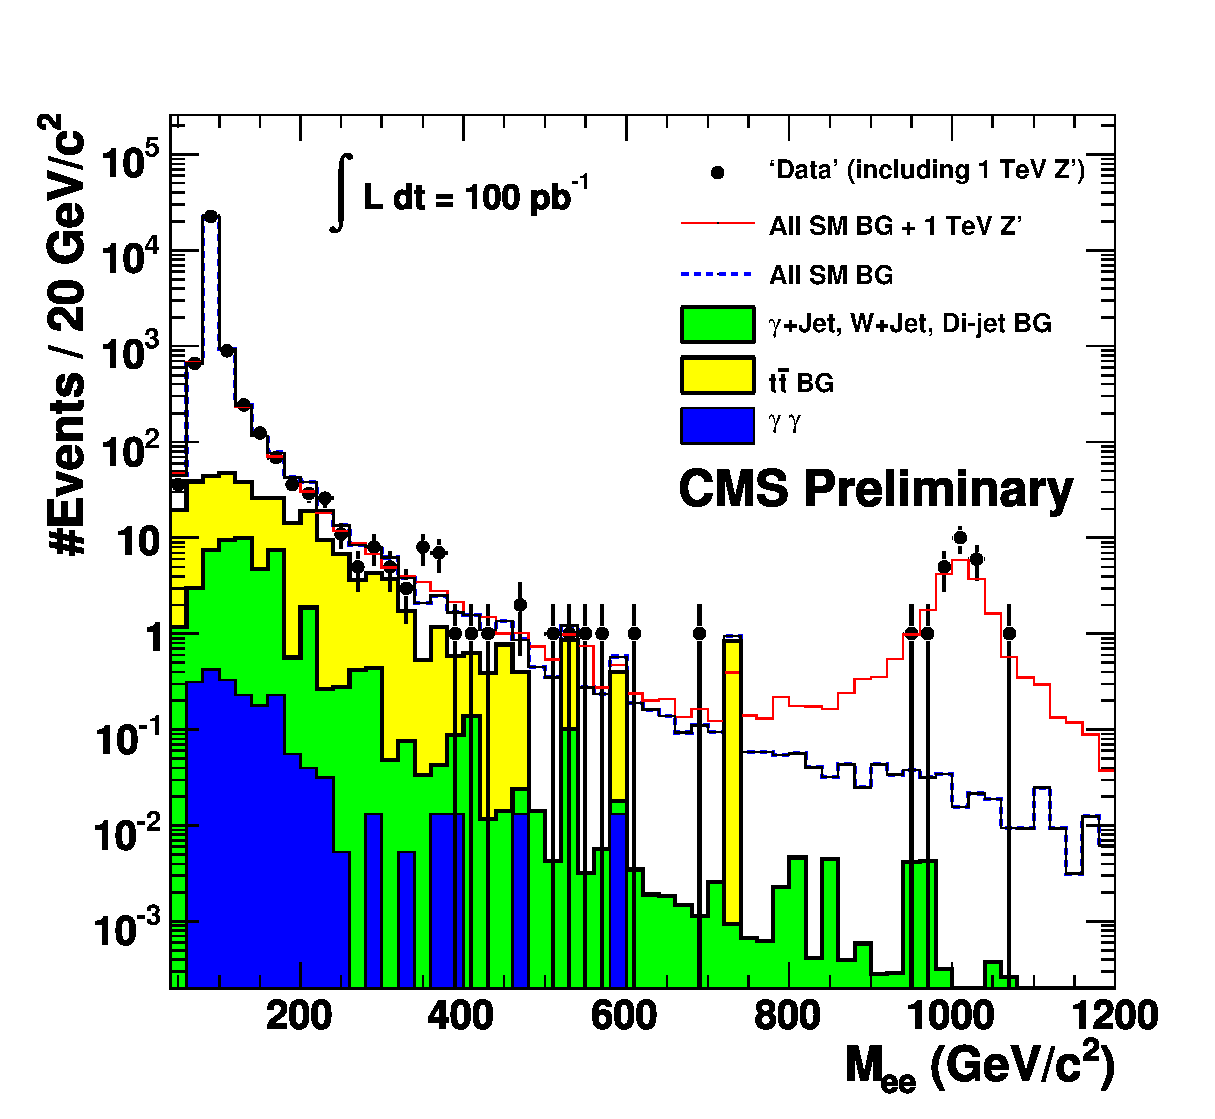
\includegraphics[width=0.45\textwidth]{./st_mass_all_withZPrime_ALLTOPO.eps}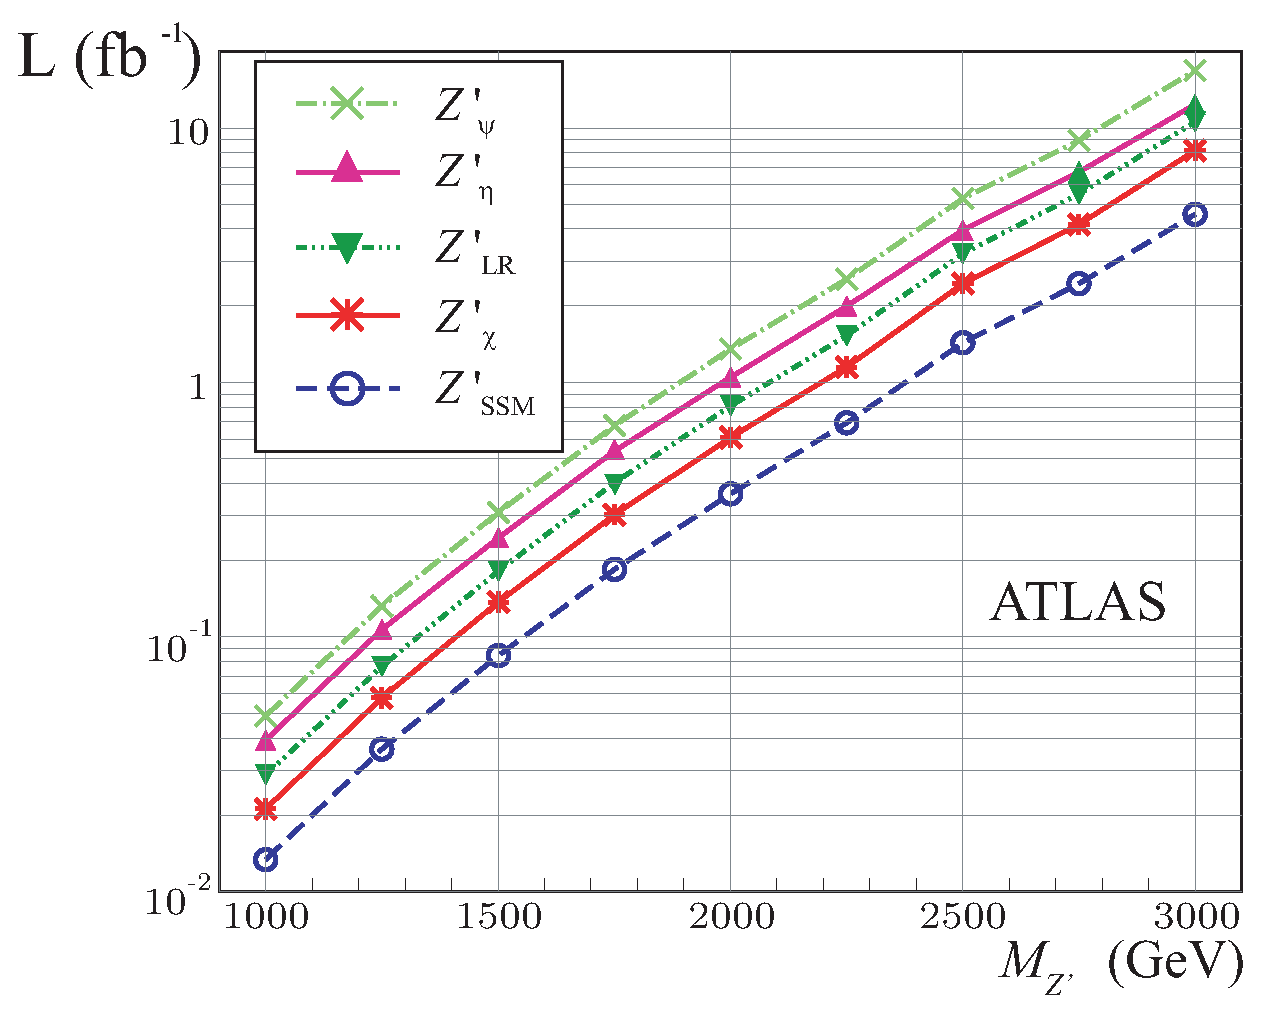
\includegraphics[width=0.48\textwidth]{./fig9L.eps}
\caption{Left: di-electron invariant mass spectrum for a 
100~pb$^{-1}$ pseudo-experiment (from CMS) including a signal from 
$Z' \rightarrow ee$ with mass of 1~TeV/$c^2$, 
compared to SM background estimates. Right: integrated 
luminosity needed for a $5\sigma$ discovery of $Z' \rightarrow ee$
as a functionof the $Z'$ mass for various benchmark models. Only 
statistical uncertainties are included. 
Effect of systemtic uncertainties is less than 20\% in the $Z'$ mass
range investigated.}
\label{fig:MeeAndZPrimeDisc}
\end{figure}

\section{Di-jet channel} \label{dijet}
The LHC is a parton-parton collider in a previously 
unexplored energy region. If new parton-parton resonances 
exist then the LHC will produce them copiously. 
These resonances should also decay to partons giving two jets in the final state. 
Therefore the experimental motivation to search for di-jet 
resonances is intuitively obvious. In addition several theoretical 
models supports the search of new physics in the di-jet channel
(FIXME - ADD REFERENCE). Even if the LHC energy is not sufficient 
to directly produce these particles, the new physics might appear as 
a contact interaction (FIXME - ADD REFERENCE), 
and we should still be able to identify its signals by looking 
at di-jet events.

Several experimental approaches have been considered by the 
ATLAS~\footnote{Results from ATLAS analysis were not yet public at the time 
of the conference, and therefore not included in this paper.} 
and CMS analyses to identify new physics in the di-jet channel, 
including the study of the jet $p_{T}$ spectrum, di-jet mass, and di-jet ratio.
In this section, the use of di-jet ratio to identify the presence 
of contact interactions is discussed. The most sensitive 
search for quark contact interactions at the Tevatron obtained an exclusion on 
the contact interaction scale of $\Lambda^{+} < 2.7$~TeV (FIXME - ADD REFERENCE - 
CHECK LATEST NUMBERS).  

The di-jet ratio $R$ is a jet angular variable used to 
discriminate between new physics and QCD multi-jet events, 
that constitute the dominant SM background in the di-jet channel:  
$R=N\mbox{(}|\eta|<0.7\mbox{)}~/~N\mbox{(}0.7<|\eta|< 1.3 \mbox{)}$, 
where $N$ is the number of di-jet events with both jets satisfying the 
$|\eta|$ pseudorapidity requirements in parenthesis.
Figure~\ref{fig:DiJetRatio} shows the sensitivity of this measurements to 
contact interactions for different values of $\Lambda^{+}$; 
with 100~pb$^{-1}$ of data contact interaction with
$\Lambda^{+} < 6.8$~TeV can be discovered, 
which is well above the current Tevatron limits.
 

\begin{figure}[htbp] 
\centering
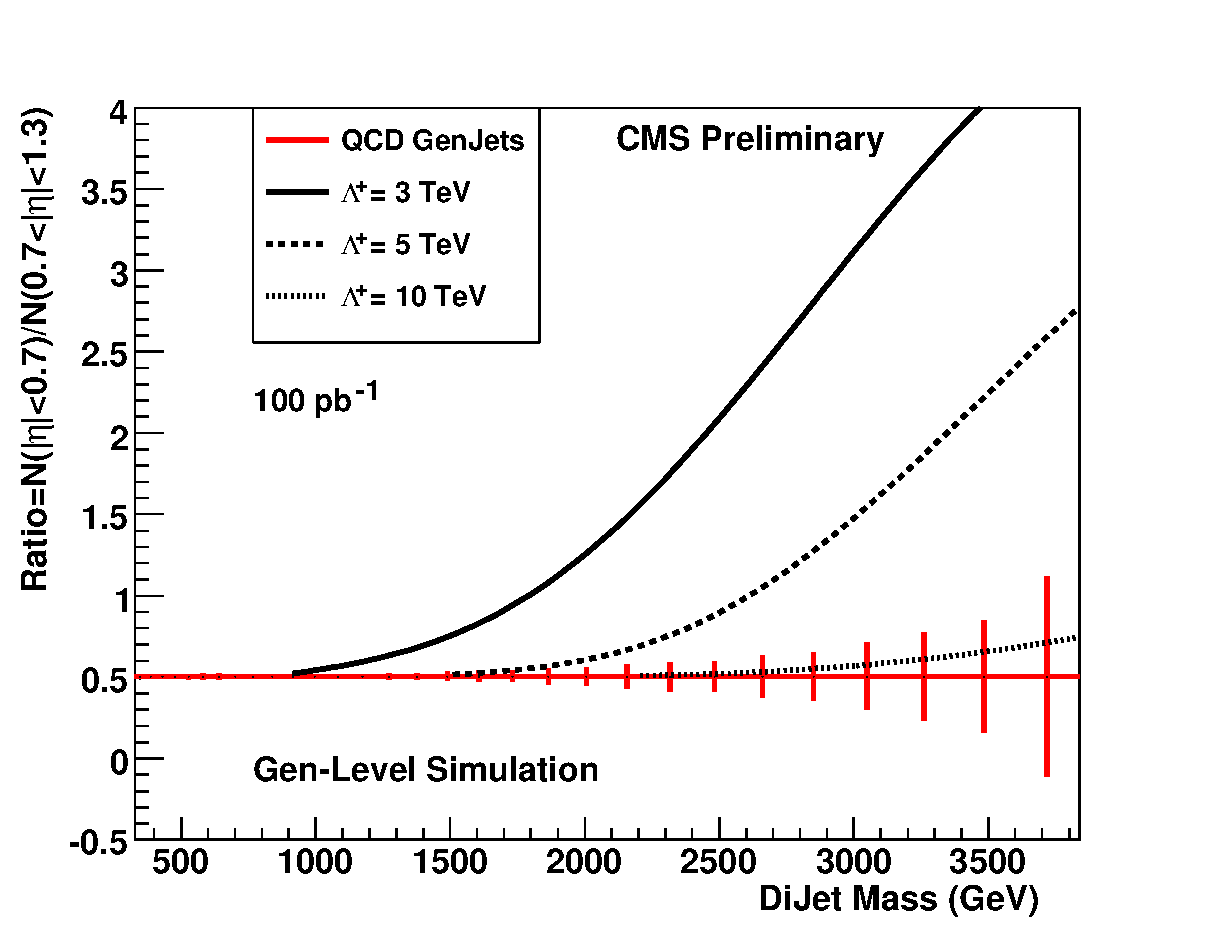
\includegraphics[width=0.45\textwidth]{./DiJetRatio100pbOptFix.eps} 
\caption{Di-jet ratio as a function of di-jet mass for contact interactions at 
different energy scales, and for QCD multi-jet background. 
For QCD multi-jet events, the di-jet ratio is almost flat at 0.5. 
In presence of contact interactions, 
leading jets are expected to be more central than QCD multi-jet events, 
thus producing a deviation in the di-jet ratio at high di-jet mass values.}
\label{fig:DiJetRatio}
\end{figure}

\section{Lepton-jet channel} \label{leptonjet}

\section{Heavy stable charged particles} \label{HSCP}

\section{Discovery potential - 10 TeV {\it vs} 14 TeV} \label{10TeVvs14TeV}

\section{Conclusion} \label{Conclusion}










%\texttt{cimento}.

%\begin{figure}
%\includegraphics{foo}     % includes figure foo.eps
%\caption{Foo onteracting with bar}
%\end{figur

%This sample is not meant to provide documentation for the class;
%to obtain the class `manual' typeset the main distribution file,
%\texttt{cimento.dtx}.

%You can also use this file as a template for your own paper:
%copy it to another filename and then modify as needed.

%\section{Examples}

%\subsection{Tables}
%Tables~\ref{tab:pricesI}, \ref{tab:pricesII} and~\ref{tab:pricesIII}
%inserted at this point.

%\begin{table}
%  \caption{Again, this time with \texttt{narrowtabular}}
%  \label{tab:pricesIII}
%  \begin{narrowtabular}{2cm}{rcl}
%    \hline
%      Ice-cream      & !1500   & lire    \\
%      More ice-cream & 15000   & lire    \\
%      Crocodile      & !1500   & dollars \\
%    \hline
%      Phone call     & !.25    & dollars \\
%      X-Men          & 1.25    & dollars \\
%      Dollar         & 1?{.}!! & dollars \\
%    \hline
%  \end{narrowtabular}
%\end{table}


%\subsection{Mathematics}
%Here is a lettered array~(\ref{e.all}), with eqs.~(\ref{e.house})
%and~(\ref{e.phi}):
%\begin{eqnletter}
% \label{e.all}
% \drm x_\sy{F} & = & 1.2\cdot10^3\un{cm}, \qquad
%                     \tx{where\ } \sy{F} = \tx{Fermi}    \label{e.house}\\
% \phi_i        & = & i\pi                                \label{e.phi}
%\end{eqnletter}

%\subsection{Citations}
%We're almost done, just some citations~\cite{ref:apo}
%and we will be over~\cite{ref:pul,ref:bra}.


%\appendix

%\section{}
%Let us go then, you and I\ldots

\acknowledgments
ADD HERE

\begin{thebibliography}{0}
\bibitem{ref:apo} \BY{Boccaccio~G. \atque de~Cam\~oes~L.}
  \IN{Phys. Rev. A}{13}{1999}{12};
  \SAME{69}{999}{1666}.
\bibitem{ref:pul} \BY{Pulci~L.}
  preprint INFN 8181.
\bibitem{ref:bra} \BY{Bragg~B.}
  \TITLE{Tender comrade},
  in \TITLE{Workers Playtime},
                  edited by \NAME{Tizio A. \atque Caio B.}
                  (Unexeditor, Bologna) 1997, pp.~1-10.
\end{thebibliography}

\end{document}
\endinput
%%
